\documentclass[12pt,a4paper]{scrartcl}
\usepackage[utf8]{inputenc}
%\usepackage[latin1]{inputenc} %  Alternativ unter Windows
\usepackage[T1]{fontenc}
\usepackage[paper=a4paper,
left=25mm,
right=25mm,
top=25mm,
bottom=20mm]{geometry}
\usepackage[nottoc]{tocbibind}
\usepackage[ngerman]{babel}
\usepackage[pdftex]{graphicx}
\usepackage{latexsym}
\usepackage{amsmath}
\usepackage{amssymb,amsthm,amsfonts}
\usepackage{mathtools}
\usepackage{enumitem}
\usepackage[utf8]{inputenc}
\usepackage{float}
\usepackage{physics}
\usepackage{subfigure}
\usepackage{wasysym}
\usepackage{amssymb}
\newcommand{\R}{\mathbb{R}}


\DeclareMathOperator{\dive}{div}
\newtheorem{Satz}{Satz}[section]\newtheorem{Definition}[Satz]{Definition} 
\newtheorem{Lemma}{Lemma}		                 
\newtheorem{Korollar}[Satz]{Korollar}
\newtheorem{Proposition}[Satz]{Proposition}                  
\newtheorem{examples}[Satz]{Beispiel}
\let\oldexamples\examples
\renewcommand{\examples}{\oldexamples\normalfont}
\newtheorem*{notation}{Notation}
\let\oldnotation\notation
\renewcommand{\notation}{\oldnotation\normalfont}
\newtheorem*{remark}{Bemerkung}
\let\oldremark\remark
\renewcommand{\remark}{\oldremark\normalfont}                  
\newtheorem*{define}{Definition}
\let\olddefine\define
\renewcommand{\define}{\olddefine\normalfont}
\newtheorem*{repetition}{Wiederholung}
\let\oldrepetition\repetition
\renewcommand{\repetition}{\oldrepetition\normalfont}

\usepackage{bbm}
\usepackage[german=quotes]{csquotes}
\usepackage{xcolor}
\newcommand*\diff{\mathop{}\!\mathrm{d}}
\DeclareMathOperator{\conv}{conv}
\DeclareMathOperator{\spann}{span}
\DeclareMathOperator{\Jacobi}{D}
\DeclareMathOperator{\diam}{diam}
\definecolor{Mygreen}{RGB}{0,128,0}
\newcommand{\defi}[1]{\textcolor{Mygreen}{#1}}
%\renewcommand{\phi}{\varphi}
\renewcommand{\epsilon}{\varepsilon}
\newcommand{\unklar}[1]{\textcolor{blue}{#1}}
\newcommand\restr[2]{{% we make the whole thing an ordinary symbol
		\left.\kern-\nulldelimiterspace % automatically resize the bar with \right
		#1 % the function
		\vphantom{\big|} % pretend it's a little taller at normal size
		\right|_{#2} % this is the delimiter
}}
\newcommand{\cupdot}{\mathbin{\mathaccent\cdot\cup}}
\DeclareMathOperator{\sign}{sign}
\newcommand{\rhoin}{\rho_{\text{in}}}
\newcommand{\Gammain}{\Gamma_{{\text{in}}}}
\newcommand{\Gammaout}{\Gamma_{{\text{out}}}}
\DeclareMathOperator{\lTG}{(TG)}
\DeclareMathOperator{\swlTG}{(swTG)}
\DeclareMathOperator{\stlTG}{(stTG)}
\DeclareMathOperator{\Abb}{Abb}
\DeclareMathOperator{\supp}{supp}

\numberwithin{equation}{section} 


% Praktikumsbericht nummer setzen
\newcommand{\BerichtNR}{3}

\begin{document}
\begin{titlepage}
	
\includegraphics[scale=0.5]{kit-logo.jpg} 
	\begin{center} 
		\LARGE 
		\vspace*{2cm}
		\LARGE Praktikumsbericht \BerichtNR
		\vspace*{1.0cm}
		\hrule
		\vspace*{0.2cm}
		{\vspace{0.2cm} \huge Einführung in das Wissenschaftliche Rechnen}\vspace{0.5cm}
		\hrule
		\vspace*{2.5cm}
		\Large Stefan Karch \\
		Florian Döttling \\
		Tim Buchholz  \\
		\vspace*{1cm}
		20.05.2019 \\
		\vspace*{1.5cm}
		\vspace*{4.0cm}
		\Large Betreuung: Prof. Dr. Christian Wieners, Niklas Baumgarten \\[0.5cm]
		\Large Fakultät für Mathematik \\
		\Large Karlsruher Institut für Technologie
	\end{center}
\end{titlepage}

\tableofcontents

\section{Zusammenfassung: lineare Transportgleichung}
% !TeX root = Bericht_main.tex
\subsection{Analytische Betrachtung der linearen Transportgleichung}
\textbf{Bisher} wollten wir aus gegebenen Randwerten den Fluss $ q $ berechnen.\\
\textbf{Jetzt} ist $ \Omega \subseteq \R^2 $ (wir betrachten nur zweidimensionale Gebiete) der Fluss $ q: \Omega \to \R^2 $ mit $ \dive(q) = 0 $ gegeben. Gesucht wird nun die Dichteverteilung $ \rho: \Omega \times [0,T] \to \R_{\geq 0} $ einer 
transportierten Substanz. Gegeben ist dazu die \defi{Anfangsverteilung} der Substanz $ \rho_0:  \Omega \to \R_{\geq 0}$ und der \defi{Einfluss} der Substanz über die Zeit $ \rhoin: \Gammain \times [0,T] \to \R_{\geq 0} $ mit $ \Gammain \coloneqq \{ z \in \partial \Omega: q(z) \cdot \nu(x) \leq 0 \} $ ($ \Gammain $ ist gerade die Menge der Randpunkte an dem Substanz einfließen kann).

Gegebenenfalls betrachten wir $ \rho $ auch als 
\[ \rho: [0,T] \to \Abb(\Omega, \R_{\geq 0}), t \mapsto \rho(\cdot,t). \]

Nach der physikalischen Modellierung gilt folgende Bilanzgleichung:
\begin{gather*}
	\forall \ K \subseteq \Omega, t \in [0,T]: \frac{\diff}{\diff t} \int_K \rho(x,t) \diff x + \oint_{\partial K} \rho(x,t) q(x) \cdot \nu(x) \diff a = 0 \\
	\stackrel{\text{Gauß}}{\implies} \int_K \partial_t \rho(x,t) + \dive(\rho q)(x,t) \diff x = 0 
\end{gather*}
Da $ K \subseteq \Omega $ beliebig ist und \unklar{$ \rho, q \in C^1(\Omega) $} folgt die \defi{lineare Transportgleichung}
\begin{gather*}
	\partial_t \rho + \dive(\rho q) = 0 \text{ in } \Omega \times (0,T) 
\end{gather*}
Mit der Randbedingung $ \rho(x,t) = \rhoin(x,t) \text{ auf } \Gammain \times (0,T)$ und der Anfangsbedingung $ \rho(x,0) = \rho_0(x) \text{ auf } \Omega $ folgt das zu lösende analytische Problem
\begin{gather*}
	\text{Bestimme } \rho: \Omega \times [0,T] \to \R_{\geq 0} \text{, sodass}\\
	\lTG
	\begin{cases}
		\partial_t \rho + \dive(\rho q) = 0 &\text{ in } \Omega \times (0,T)\\
		\rho(x,t) = \rhoin(x,t) &\text{ auf } \Gammain \times ()0,T)\\
		\rho(x,0) = \rho_0(x) &\text{ auf } \Omega
	\end{cases}
\end{gather*}


\newpage
\subsection{Erhaltungsgrößen der analytischen Lösung}
\label{subsec:Erhaltungsgroessen der analytischen Loesung}
\begin{Lemma}[Massenbilanz]
	\label{Massenbilanz}
	
	Sei $ \rho $ Lösung von $ \lTG $. 
	
	Dann gilt die \defi{Massenbilanz}:
	\[ \underbrace{\int_{\Omega} \rho(x,t) \diff x}_{(1)} = \underbrace{\int_{\Omega} \rho_0(x) \diff x}_{(2)}  \underbrace{-\int_{0}^{t} \int_{\Gammain} \rhoin(x,\tilde{t}) q(x) \cdot \nu(x) \diff a \diff \tilde{t}}_{(3)} \underbrace{- \int_{0}^{t} \int_{\Gammain} \rho(x,\tilde{t}) q(x) \cdot \nu(x) \diff a \diff \tilde{t}}_{(4)} \]
\end{Lemma}
	Interpretation der Terme:
	\begin{enumerate}[label=(\arabic*)]
		\item Masse zum Zeitpunkt $ t $,
		\item Masse zum Anfangszeitpunkt $ 0 $,
		\item Masse, die in $ [0,t] $ hinzu geflossen ist ($ \nu $ ist äußere Normale, deswegen \enquote{-} statt \enquote{+}),
		\item Masse, die in $ [0,t] $ abgeflossen ist.
	\end{enumerate}

\begin{Lemma}[Energiebilanz]
	\label{Energiegleichung}
	
	Sei $ \dive(q) = 0 $ und $ \rho $ eine Lösung von $ \lTG $. 
	
	Dann gilt die \defi{Energiebilanz}: $ \forall \ t\in [0,T] $
	\[\int_{\Omega} \abs{\rho(x,t)}^2 \diff x = \int_{\Omega} \abs{\rho_0(x)}^2 \diff x  + \int_{0}^{T} \left[ \int_{\Gammain}\abs{\rhoin(t)}^2 \abs{q\cdot n} \diff a - \int_{\Gammaout} \abs{\rho(t)}^2 \abs{q\cdot n} \diff a  \right] \]
\end{Lemma}

\subsection{Lösungsbegriffe von $ \lTG $}

\begin{define}(Lösungsbegriffe)
	
	\begin{itemize}
		\item Eine Lösung von
		\begin{gather*}
		\text{Bestimme } \rho: \Omega \times [0,T] \to \R_{\geq 0} \text{, sodass}\\
		\lTG
		\begin{cases}
		\partial_t \rho + \dive(\rho q) = 0 &\text{ in } \Omega \times (0,T)\\
		\rho(x,t) = \rhoin(x,t) &\text{ auf } \Gammain \times (0,T)\\
		\rho(x,0) = \rho_0(x) &\text{ auf } \Omega.
		\end{cases}
		\end{gather*}
		heißt \defi{klassische Lösung}.
%		\item Eine Lösung von 
%		\begin{gather*}
%		\text{Bestimme } \rho: \Omega \times [0,T] \to \R_{\geq 0} \text{, sodass}\\
%		\stlTG
%		\begin{cases}
%		\int_{\Omega} \int_{0}^{T} \partial_t \rho + \dive(\rho q) \phi \diff t \diff x = 0 &\text{ in } \Omega \times (0,T)\\
%		\rho(x,t) = \rhoin(x,t) &\text{ auf } \Gammain \times (0,T)\\
%		\rho(x,0) = \rho_0(x) &\text{ auf } \Omega
%		\end{cases}\\
%		\text{ für alle } \phi: \Omega \times (0,T) \to \R.
%		\end{gather*}
%		heißt \defi{starke Lösung}.
		\item Eine Lösung von 
		\begin{gather*} 
		\text{Bestimme } \rho \in L^1(\Omega \times [0,T], \R_{\geq 0}) \text{, sodass}\\
		\swlTG
		\begin{cases}
		\displaystyle
		\int_{\Omega} \rho_0 \phi(0) \diff x = \mkern-16mu &- \displaystyle \int_{0}^{T} \int_{\Omega} \rho (\partial_t \phi - q \nabla_{\unklar{x}} \phi ) \diff x \diff t \\
		&+\displaystyle\int_{0}^{T} \left[ \oint_{\Gammain} \rhoin q \cdot \nu \phi \diff a + \oint_{\Gammaout} \rho q \cdot n \phi \diff a \right] \diff t
		\end{cases}	\\
		\unklar{\text{ für alle } \phi: \Omega \times (0,T) \to \R \text{ mit } \phi(\cdot,T) = 0 \text{ auf } \Omega \text{ und } \phi = 0 \text{ auf } \Gammain \times (0,T).}
		\end{gather*}
		heißt \defi{schwache Lösung}.
	\end{itemize}
\end{define}

\begin{Lemma}(Zusammenhang der Lösungsbegriffe)
	
	\begin{enumerate}
		\item Ist $ \rho $ eine klassische Lösung, so ist $ \rho $ auch eine schwache Lösung.
		\item Ist $ \rho $ glatt genug und eine schwache Lösung, so ist $ \rho $ eine klassische Lösung. 
	\end{enumerate}
\end{Lemma}

\subsection{Numerische Approximation}
Ziel ist es nun eine \enquote{gute} Approximation für die schwache Lösung $ \rho $ von $ \swlTG $ zu finden. Dabei werden wir $ \rho $ zunächst im Raum diskretisieren um die semi-diskrete Lösung $ \rho_h $ zu erhalten. Anschließend diskretierien wir in der Zeit.

\subsubsection{Diskretisierung im Raum}
\unklar{Wir betrachten $ \rho $ als Lösung und schreiben das zu lösende Problem um.} Sei $ \mathcal{K} $ eine Triangulierung von $ \Omega $ wie bisher und $ (\cdot,\cdot)_A $ das $ L^2(A) $-Skalarprodukt. 
\begin{define}(Flux)
	
	Zu gegebenen Fluss $ q:\Omega \to \R^2 $ definieren wir die \defi{Flussfunktion}/\defi{Flux} als
	\[ \Psi: \Abb(\Omega \times [0,T], \R) \to \Abb(\Omega \times [0,T], \R^2), \Psi(\rho) = \rho q \]
\end{define}

Dann gilt für eine klassische Lösung $ \rho $ von $ \lTG $  $ \partial_t \rho = - \dive(\Psi(\rho)) $ und somit
\begin{align*}
	&&&\sum_{K \in \mathcal{K}} \oint_{\partial K} \phi \Psi(\rho) \cdot n^K \diff a \stackrel{(\star)}{=} \oint_{\partial \Omega} \phi \Psi(\rho) \cdot n \diff a \stackrel{\text{Gauß}}{=} \int_{\Omega} \dive(\Psi(\rho) \Phi) \diff x \\
	&&& \quad = \int_{\Omega} \phi \dive(\Psi(\rho)) + \Psi(\rho) \cdot \nabla \phi \diff x = - \int_\Omega \partial_t \rho \phi \diff x + \int_\Omega \Psi(\rho) \cdot \nabla \phi \diff x \\
	&\iff &&\sum_{K \in \mathcal{K}} \left(\Psi(\rho) \cdot n^K, \phi \right)_{\partial K} = - \left(\partial_t \rho, \phi  \right)_\Omega - \left(\Psi(\rho), \nabla\phi  \right)_\Omega \\
	&\iff && \left(\partial_t \rho, \phi  \right)_\Omega  = - \left(\Psi(\rho), \nabla\phi  \right)_\Omega - \sum_{K \in \mathcal{K} } \left(\Psi(\rho) \cdot n^K, \phi \right)_{\partial K} \\
	&\iff &&\left(\partial_t \rho, \phi  \right)_\Omega  = - \left(\Psi(\rho), \nabla \phi  \right)_\Omega - \sum_{K \in \mathcal{K}} \sum_{F \in \mathcal{F}_K} \left(\Psi(\rho) \cdot n^K, \phi \right)_{F} \\
	&\stackrel{\mathclap{\substack{\text{Kanten} \\ \text{Nullmengen}}}}{\iff} &&\sum_{K \in \mathcal{K}} \left(\partial_t \rho, \phi  \right)_K  = - \left(\Psi(\rho), \nabla \phi  \right)_\Omega - \sum_{K \in \mathcal{K}} \sum_{F \in \mathcal{F}_K} \left(\Psi(\rho) \cdot n^K, \phi \right)_{F} \\
	&\iff  &&\sum_{K \in \mathcal{K}} \left(\partial_t \rho, \phi  \right)_K  = \sum_{K \in \mathcal{K}} \bigg( - \left(\Psi(\rho), \nabla \phi \right)_K\\
	&&&\qquad\qquad\qquad\qquad -\sum_{\substack{F \in \mathcal{F}_K \\ F \not\subseteq \Gammain}} \left(\Psi(\rho) \cdot n^K, \phi \right)_{F}- \sum_{\substack{F \in \mathcal{F}_K \\ F \subseteq \Gammain}} \left(\rhoin q \cdot n^K, \phi \right)_{F} \bigg)\\
	&\iff  &&\sum_{K \in \mathcal{K}} \left(\partial_t \rho, \phi  \right)_K  = \sum_{K \in \mathcal{K}} \bigg( -\left(\Psi(\rho), \nabla\phi \right)_K \\
	&&& \qquad\qquad\qquad\qquad -\sum_{\substack{F \in \mathcal{F}_K \\ F \not\subseteq \Gammain}} \left(\Psi(\rho) \cdot n^K, \phi \right)_{F} - \left(\rhoin q \cdot n^K, \phi \right)_{\partial K \cap \Gammain} \bigg) \tag{\sun}
\end{align*}
\begin{remark}
	zu $ (\star) $: Integration über inneren Kanten $ F $ fällt weg, da für die beiden Nachbarzellen wegen der äußeren Normalen in unterschiedliche Richtungen integriert wird:
	\[ F = K \cap K': \oint_{F}  \phi \Psi(\rho) \cdot n^K \diff a = - \oint_{F} \phi \Psi(\rho) \cdot n^{K'} \diff a\]
\end{remark}
\ \newline
\textbf{Ziel}:
Wir wollen nun die semidiskrete Lösung $ \rho_h: [0,T] \to Q_h $ bzw eine Differenzialgleichung für $ \rho_h $ herzuleiten. 

\textbf{Approximation}:
Wähle Lösungs-/Ansatzraum $ Q_h = \Pi_{K\in\mathcal{K}} \mathbb{P}_k $ für $ k \in \mathbb{N}_0 $. Für $ k = 0 $ heißt $ Q_h $ \defi{Finite-Volumen-Raum}, für $ k \geq 1 $ nennt man $ Q_h $ \defi{Discontinuous-Galerkin-Raum}. Anders als bei den FE-Räumen wird für Elemente aus $ Q_h $ keine Stetigkeit auf $ \Omega $ gefordert. D.h. im Allgemeinen lässt sich $ u \in Q_h $ (Definiert auf $ \Omega_h $) nicht stetig auf $ \Omega $ fortsetzen, da für eine beliebige innere Kante $ \overline{F} = \partial K \cap \partial K' $ mit Grenzwert von $ K $ aus unterschiedlich zu dem von $ K' $ aus sein kann. Damit kann (\sun) nicht direkt auf $ Q_h $ übertragen werde, da noch zu klären ist, was $ \Psi(\rho) $ auf $ F \in \mathcal{F} $ bedeutet. Wir betrachten den \defi{numerischen Fluss} (numerical flux), welcher \enquote{in geeigneter Weiße} $ \Psi(\rho) $ auf den Kanten $ F \in \mathcal{F} $ ersetzt . Wir zählen $ \mathcal{K} $ durch mit $ \mathcal{K} = \{K_1 , \dots , K_N\} $, $ N \coloneqq \abs{\mathcal{K}} $.
Unser numerischer Ansatz wird durch (\sun) motiviert und lautet für alle $ \phi_h \in Q_h $
\[
\sum_{i = 1}^{N} \left(\partial_t \rho_h, \phi_h  \right)_{K_i}  = \sum_{i=1}^{N} \bigg(- \left(\Psi(\rho_h), \nabla\phi_h \right)_{K_i} -\sum_{\substack{F \in \mathcal{F}_{K_i} \\ F \not\subseteq \Gammain}} \left(\Psi^*(\rho_h) \cdot n^K, \phi \right)_{F} - \left(\rhoin q \cdot n^K, \phi \right)_{\partial K_i \cap \Gammain} \bigg)
\]



\textbf{Finite-Volumen}:
Wir betrachten im folgenden zunächst nur den Finite-Volumen-Ansatzraum $ Q_h = \Pi_{K \in \mathcal{K}} \mathbb{P}_0 $. 

Als numerischen Fluss verwenden wir den \defi{upwind flux} $ \Psi^* $. Dieser ist gegeben für alle $ K \in \mathcal{K} $ und $ F \in \mathcal{F}_K $ durch:
\begin{gather*}
	\text{Auf } F \text{ gilt }\Psi^*(\rho_h) = \begin{cases}
	\Psi(\rho_{h|K}) &\text{, für } q \cdot n^K_{|F} > 0\\
	\Psi(\rho_{h|K'}) &\text{, für } q\cdot n^K_{|F} < 0 \text{ und } \overline{F} = \partial K \cap \partial K'\\
	0 &\text{, für } q\cdot n^K_{|F} < 0 \text{ und } F \subseteq \Gammain.
	\end{cases}  
\end{gather*}

\begin{remark}(alternativer numerischer Fluss)
	
	Eine weitere interessante Möglichkeit für den numerischen Fluss ist der \defi{central flux} $ \Psi^c $. Dieser ist gegeben für alle $ K \in \mathcal{K} $ und $ F \in \mathcal{F}_K $ durch:
	\begin{gather*}
		\text{Auf } F \text{ gilt }\Psi^c(\rho_h) = \begin{cases}
		\frac{1}{2} \left( \Psi(\rho_{h|K}) + \Psi(\rho_{h|K'}  \right) &\text{, auf } \overline{F} = \partial K \cap \partial K'\\
		\Psi(\rho_{h|K}) &\text{, auf } F \subseteq \Gammain\\
		0 &\text{, auf } F \subseteq \Gammaout 
		\end{cases}
	\end{gather*}
\end{remark}

\begin{remark}
	Wir führen einen Notation für die Nachbarzelle an einer Kante ein.
	
	Für $ K \in \mathcal{K} $ und eine innere Kante $ F \in \mathcal{F}_K $ sei $ K_F \in \mathcal{K}$ die Zelle, sodass gilt \[ \overline{F} = \partial K \cap \partial K_F \]
	
	Gilt  $q\cdot n^K_{|F} < 0$ so ist $ \Psi^*(\rho_h) = \Psi(\rho_{h|K_F}) $ auf der inneren Kante $ F $.
\end{remark}
\bigskip
Weiter gilt für die Zellenbasis $ \{\mu_i\}_{i=1}^N $ mit $ \mu_i = \mathbbm{1}_{K_i} $ 
\begin{itemize}
	\item $ Q_h = \spann\{\mu_1, \dots , \mu_N\} $,
	\item \unklar{$ \{\mu_i\}_{i=1}^N $ ist eine Orthogonalbasis (im Allegemine aber keine ONB da $ \norm{\mu_i}^2 = \lambda(K_i) $\,),}
	\item $ \forall \ i \in \{1, \dots , N\}:  \supp(\mu_i) \subseteq \overline{K_i}$.
\end{itemize}
 
Durch Einsetzen der Zeilenbasis und mit $ \supp(\mu_i) \subseteq \overline{K_i} (\ i \in \{1, \dots , N\})$ ergibt sich für alle $\ i \in \{1, \dots , N\}$ 
\begin{align*}
	\left(\partial_t \rho_h, \mu_i  \right)_{K_i}  &= \bigg( -\underbrace{(\Psi(\rho_h), \nabla\mu_i)_{K_i}}_{=0 \text{, da } \nabla \mu_i = 0} - \sum_{\substack{F \in \mathcal{F}_{K_i} \\ F \not\subseteq \Gammain}} \left(\Psi^*(\rho_h) \cdot n^{K_i}, \mu_i \right)_{F} - \left(\rhoin q \cdot n^{K_i}, \mu_i \right)_{\partial K_i \cap \Gammain} \bigg) \\
	&= \bigg( - \sum_{\substack{F \in \mathcal{F}_{K_i}, F \not\subseteq \Gammain\\ F \text{ mit }q \cdot n^K_{|F} > 0} } \left(\underbrace{\Psi^*(\rho_h)}_{= \rho_{h|K}\, q} \cdot n^{K_i}, \mu_i \right)_{F} - \sum_{\substack{F \in \mathcal{F}_{K_i}, F \not\subseteq \Gammain\\ F \text{ mit }q \cdot n^K_{|F} < 0} } \left(\underbrace{\Psi^*(\rho_h)}_{= \rho_{h|K_F} \, q} \cdot n^{K_i}, \mu_i \right)_{F}\\
	& \qquad \qquad \qquad \qquad \qquad \qquad  \qquad \qquad\qquad \qquad- \left(\rhoin q \cdot n^{K_i}, \mu_i \right)_{\partial K_i \cap \Gammain} \bigg)\qquad \qquad
\end{align*} 

Zusammen mit der Basisdarstellung von $ \rho_h $ in $\{\mu_i  \}_{i=1}^N$, $ \rho_h = \sum_{i=1}^{N} \underline{\rho}[i] \; \mu_i$, und 
\begin{align*}
&\text{\defi{Massenmatrix} } \underline{M}\in \R^{N \times N} \\  &\qquad \qquad \underline{M}[K,K'] \coloneqq \begin{dcases}
\int_K \abs{\mu_K}^2 \diff x & \text{, für } K = K' \\
0 &\text{, sonst}
\end{dcases} \\
&\text{\defi{Flussmatrix} } \underline{A}\in \R^{N \times N} \\ &\qquad \qquad \underline{A}[K,K'] \coloneqq \begin{dcases}
- \sum_{\substack{F\in \mathcal{F}_K \\ F \text{ mit } q\cdot n^K_{|F} > 0}} \oint_F \mu_K^2 q \cdot n^K \diff a& \text{, für } K = K' \\
- \oint_F \mu_K \mu_{K'} q \cdot n^K \diff a &\text{, für } q \cdot n^K< 0 \text{ und } \overline{F} = \partial K \cap \partial K'\\
0 &\text{, sonst}
\end{dcases} \\
&\text{\defi{Lastvektor} } \underline{b}\in \R^{N} \\ &\qquad \qquad\underline{b}[K] \coloneqq \oint_{\partial K \cap \Gammain} \rhoin q \cdot n \diff a
\end{align*}


ergibt sich die DGL
\begin{gather*}
\begin{cases}
\underline{M} \partial_t \underline{\rho} = \underline{A} \underline{\rho} + \underline{b} \\
\underline{\rho}(0) = \underline{\rho_0}
\end{cases}\\
\implies \underline{\rho}(t) = \exp(t \underline{M}^{-1} \underline{A}) \left( \underline{\rho_0} + \int_{0}^{t} \exp(-s\underline{M}^{-1} \underline{A}) b(s) \diff s \right) 
\end{gather*}

\subsubsection{Diskretisierung in der Zeit}

Wir wollen in diesem Kapitel noch auf die Herleitung der Zeitintegratoren eingehen. Der Ansatz hierbei besteht aus der 
Integration der Differentialgleichung $\underline{M} \partial_t \underline{\rho} = \underline{A} \underline{\rho} + \underline{b}$ über die Zeit $t$ im Intervall $[t_i, t_{i+1}]$.
Dabei ist $t_i = i \Delta t$. Hiermit folgt:
\begin{align*}
  \underline{M}\underline{\rho}(t_{i+1}) - \underline{M}\underline{\rho}(t_i) = \int_{t_i}^{t_{i+1}}
  \underline{M} \partial_t \underline{\rho}(t) dt =\int_{t_i}^{t_{i+1}} \underline{A} \underline{\rho}(t) + \underline{b} dt.
\end{align*}
Mithilfe der Anwendung verschiedener Quadraturformeln lässt sich daraus ein Runge-Kutta Verfahren herleiten. Über die Rechteckformel 
\begin{align*}
  \int_{t_i}^{t_{i+1}}\underline{A} \underline{\rho}(t) + \underline{b} dt \approx (t_{i+1}-t_i) 
  \underline{A} \underline{\rho}(t_i+1) + \underline{b} = \Delta t \underline{A} \underline{\rho}(t_{i+1}) + \underline{b}
\end{align*}
ergibt sich z.B. das implizite Euler Verfahren
\begin{align*}
  \underline{\rho}(t_{i+1}) = \underline{\rho}(t_{i}) + \Delta t \underline{M}^{-1}\underline{A} \underline{\rho}(t_{i+1}) + \underline{b}.
\end{align*}
Weitere Verfahren, die wir verwenden werden, sind zum einen das
klassische Runge-Kutta Verfahren
\begin{align*}
  \underline{\rho}(t_{i+1}) = \underline{\rho}(t_{i}) +
  \Delta t \underline{M}^{-1}\underline{A} (
  \underline{\rho}(t_{i}) +
  \frac{\Delta t}{2} \underline{M}^{-1}\underline{A} (
  \underline{\rho}(t_{i}) +
  \frac{\Delta t}{3} \underline{M}^{-1}\underline{A} (
  \underline{\rho}(t_{i}) +
  \frac{\Delta t}{4} \underline{M}^{-1}\underline{A} 
  \underline{\rho}(t_{i}) )))
\end{align*}
und zum anderen die implizite Mittelpunktsregel 
\begin{align*}
  \underline{\rho}(t_{i+1}) = \underline{\rho}(t_{i}) +
  \Delta t \underline{M}^{-1} (
  \underline{A} 
  \frac{1}{2}(\underline{\rho}(t_{i}) +
  \underline{\rho}(t_{i+1}) )
  +
  \frac{1}{2} ( \underline{\rho}(t_{i}) +
  \underline{\rho}(t_{i+1}) )).
\end{align*}

\subsection{Erhaltungsgrößen der numerischen Lösung}

\begin{repetition}
	Wie in Abschnitt \ref{subsec:Erhaltungsgroessen der analytischen Loesung} \enquote{Erhaltungsgrößen der analytischen Lösung} gesehen gilt für die analytische Lösung:
	\begin{itemize}
		\item nicht-negativ (da der Zielraum von $ \rho: \Omega \times [0,T] \to \R_{\geq 0}$ $ \R_{\geq 0} $ ist)
		\item Massenbilanz (Lemma \ref{Massenbilanz})
		\item Endergiebilanz (Lemma \ref{Energiegleichung})
	\end{itemize}
\end{repetition}

Wir interessieren uns, in wie weit diese Eigenschaften der analytischen Lösung $ \rho $ von der semi-diskreten Lösung $ \rho_h $ erhalten werden.


 
\begin{Lemma}[diskrete Nicht-Negativität] \label{disktrete Nicht-Negativität}
		Sei $ q = q_h \in W_h, \dive(q) = 0 $ und $ \rho_0 \in Q_h $.$ \unklar{(?)} $ %Es gelten die gleichen Voraussetzungen wie in Lemma \ref{diskrete Massenbilanz}.
	
	Dann gilt für die semidiskrete Approximation $ \rho_h \in Q_h$ mit \enquote{upwind flux} die \defi{diskrete Nicht-Negativität}:
	\[ \rho_0 \geq 0 \text{ und } \rhoin \geq 0 \implies \rho_h \geq 0 \]
\end{Lemma}

\begin{Lemma}[diskrete Massenbilanz] \label{diskrete Massenbilanz}
	Es gelten die gleichen Voraussetzungen wie in Lemma~\ref{disktrete Nicht-Negativität}.
	
	Dann gilt für die semidiskrete Approximation $ \rho_h \in Q_h$ mit \enquote{upwind flux} oder mit \enquote{central flux} die \defi{diskrete Massenbilanz}:
	\[\forall t \in [0,T]: \int_\Omega \rho_h(t) \diff   = \int_\Omega \rho_0 \diff x - \int_{0}^{t} \left( \oint_{\Gammain} \rhoin(\tilde{t}) q \cdot n \diff a + \oint_{\Gammaout} \rho_h(\tilde{t}) q \cdot n \diff a  \right) \diff \tilde{t} \]
\end{Lemma}

\begin{Lemma}[diskrete Energiebilanz] \label{diskrete Energiebilanz}	Es gelten die gleichen Voraussetzungen wie in Lemma~\ref{disktrete Nicht-Negativität}.
	
	Dann gilt für die semidiskrete Approximation $ \rho_h \in Q_h $ mit \enquote{central flux} die \defi{diskrete Energiebilanz}:
	
	\begin{gather*}
		\forall t \in [0,T]: \int_\Omega \abs{\rho_h(t)}^2 \diff x = \int_\Omega \abs{\rho_0}^2 \diff x + \int_{0}^{\unklar{t}} \left[ \oint_{\Gammain} \abs{\rhoin(\tilde{t})}^2 \abs{q \cdot n} \diff a - \oint_{\Gammaout} \abs{\rho_h(t)}^2 \abs{q \cdot n} \diff a \right. \\
		\left. - \sum_{F\in \mathcal{F} \cap \Omega^\circ} \oint_F \abs{\rho_{h|K} - \rho_{h|K_F}}^2 \abs{q \cdot n} \diff a - \oint_{\Gammain} \abs{\rho_h - \rhoin}^2 \abs{q\cdot n} \diff a \right] \diff t
	\end{gather*}
	
\end{Lemma}
 
 
 \begin{remark}(zu Lemma \ref{diskrete Energiebilanz})
 	
 	$ \mathcal{F} \cap \Omega^\circ = \mathcal{F} \cap \Omega $ ist die Menge der inneren Kanten.
 \end{remark}

\begin{remark}(zu numerischen Flüssen)
	
%	\begin{itemize}
%		\item \unklar{ Der \enquote{upwind flux} $ \Psi^* $ ist masseerhaltend, aber nicht energieerhaltend (erfüllt also die diskrete Massenbilanz, aber i. A. nicht die diskrete Energiebilanz).}
%		\item \unklar{Der \enquote{\defi{central flux}} $ \Psi^c $ gegeben durch $ \Psi^c = \frac{1}{2} \left(\Psi(\rho_{h|K}) + \Psi(\rho_{h|K_F})\right)$ ist energieerhaltend, aber nicht monoton (d.h. erfüllt i.A. nicht die diskrete Postitvität). }
%	\end{itemize}

	\begin{tabular}{c || c | c | c}
		&\enquote{upwind flux} $ \Psi^* $ & \enquote{central flux} $ \Psi^c $ & Bedeutung \\ \hline 
		Masseerhaltend & $\checkmark$ & $\checkmark$ & diskrete Massenbilanz \\ \hline
		Energieerhlatend &  x  & $ \checkmark $ & diskrete Energiebinalz\\ \hline
		Monoton & $ \checkmark $ & x & diskrete Nicht-Negativität \\
	\end{tabular}
\end{remark}
\newpage
\subsection{Discontinuous-Galerkin-Verfahren}
Wir wollen nun noch (kurz) auf das Discontinuous-Galerkin-Verfahren eingehen. Im Gegensatz zum Finite Volumen Verfahren, wollen wir uns hierbei aber auf die wesentlichen Unterschiede und Ideen beschränken und dabei auf eine vollständige Herleitung verzichten. \newline
Im Gegensatz zum Finite Volumen Verfahren wählen wir beim Discontinuous-Galerkin-Verfahren $\Pi_{K\in\mathcal{K}} \mathbb{P}_k $ mit $ k \geq 1 $. Es sei noch einmal wie bereits beim Finite-Volumen-Verfahren erwähnt, dass hierbei für die Elemente aus $Q_h$ keine Stetigkeit auf $\Omega$ gefordert wird. \newline
Anschließend bestimmen wir $\rho_h : [0,T] \rightarrow Q_h$ mit:
	\begin{align*}
		(\partial_t \rho_h , \Phi_h)_{\Omega} &= -(\Psi(\rho_h),\nabla \Phi_h)_{\Omega}
		- \sum_{K \in \mathcal{K}}(\Psi^*(\rho_h),\Phi_h)_{\partial K \setminus \Gammain}
		-(\Psi(\rho_{in}),\Phi_h)_{\Gammain} \\
		&= \sum_{K \in \mathcal{K}} [ -( \dive \Psi (\rho_h),\Phi_h)_{K}
		+ \sum_{ F \subset \partial K \setminus \Gammain} ((\Psi(\rho_h)-\Psi ^* (\rho_h)) \cdot n_k , \Phi_h)_F ] \\		
		&\qquad +(\Psi(\rho_h) - \Psi(\rho_{in}),\Phi_h)_{\Gammain} 
		+ ( \Psi(\rho_h) \cdot n , \Phi )_{ \Gammain } \\
		&\eqqcolon  (A_h \rho_h, \Phi_h )_{\Omega} + (\rho_{in} \mid qn \mid ,\Phi_h)_{\Gammain} \\
		&\eqqcolon (A_h \rho_h, \Phi_h )_{\Omega} + (b_h,\Phi_h)_{\Gammain}
	\end{align*}  
\begin{remark}
	\begin{enumerate} 
		\item Für den DG-Operator $A_h: Q_h \rightarrow Q_h'$ gilt: 	\newline
		\begin{align*}
			(A_h,\rho_h,\rho_h)_{\Omega} &= - \int_{\partial 	\Omega} | \rho_h | ^2 | q \cdot n | da - \frac{1}{2} \sum_{F 	\in \mathcal{F} \backslash \partial \Omega} | \rho_k - 	\rho_{K_f} |^2 |q \cdot n| da \\
			&\Rightarrow - \underline{A} \text{ ist positiv 	semidefinit}
		\end{align*}
		\item Lemma 5 (die diskrete Massebilanz) lässt sich auf das DG-Verfahren übertragen, indem statt punktweiser Erhaltung, Erhaltung im Mittel betrachtet wird.
		\item Es gilt für die DG-Approximation mit Upwind-Flux: \newline
		\begin{align*}
			\int_{\Omega} | \rho_h (t) | ^2 dx &= \int_{\Omega} |\rho_0 |^2 dx 
			+ \int_0^t \oint_{\Gammain} | \rho_{in} |^2 |q \cdot n | da d \tilde{t}
			- \int_0^t \oint_{\Gamma_{out}} |\rho_h |^2 |q \cdot n | da d \tilde{t} \\
			&- \sum_{F \in \mathcal{F}_h \cap \Omega^0} \int_0^t \oint_F | \rho_K - \rho_{K_f} |^2 |q \cdot n| da d \tilde{t}
			- \int_0^t \oint_F |\rho_{in} - \rho_h |^2 |q \cdot n| da d \tilde{t}
		\end{align*}
	\end{enumerate}
\end{remark}

<<<<<<< HEAD
=======
	

	


>>>>>>> 2d6d045a6b4dcd715c8c990e85f9e231e22591f9


\section{Ergebnisse der Aufgaben}
% !TeX root = Bericht_main.tex
\subsection{Aufgabe 35}
Wir betrachten nochmals das Regenwasserversickerungsproblem aus den ersten Übungsblättern und wollen im Folgenden vorallem die Genauigkeit von linearen, quadratischen und DG-Ansatzelementen
vergleichen. Dazu betrachten wir das gleiche Problem auf unterschiedlichen Leveln für die unterschiedlichen Ansätze. Wir  wollen vorallem die Größen Outflow, Flux Error, Flux Loss vergleichen und zusätzlich mit den Größen Problem Size und Programmdauer auf den Faktor Effizienz eingehen.

\subsubsection{Aufgabe 35.1}
In einem ersten Schritt wollen wir den Einfluss der Wahl der Ansatzelemente beim Finiten Elemente Verfahren untersuchen.
Wir betrachten dazu die entsprechenden Lösungen für lineare Ansatzelemente (Discretization = linear) und quadratische Ansatzelemente (Discretization = serendipity) bei ähnlicher Problemgröße.
\begin{figure}[H]
	\centering
	\captionabove{Discretization = linear}
	\subfigure{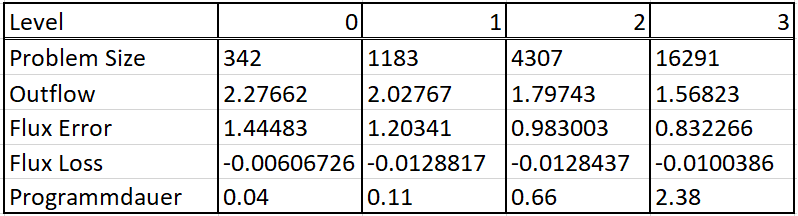
\includegraphics[width=0.99\textwidth]{../Aufgabe35/35_1_linear.png}}	 
\end{figure}

\begin{figure}[H]
	\centering
	\captionabove{Discretization = serendipity}
	\subfigure{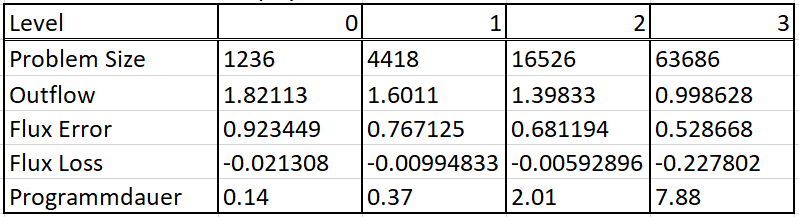
\includegraphics[width=0.99\textwidth]{../Aufgabe35/35_1_serendipity.png}}	 
\end{figure}
Man sieht sehr leicht, dass bei ähnlicher Problemgröße die quadratischen Ansatzelemente den linearen Ansatzelementen überlegen sind. Beispielsweise liefert der lineare Ansatz auf Level 1 (Problemgröße $\approx$ $1200$) einen Flux Error von $\approx 1.2$, während der quadratische Ansatz aus Level 0 (ebenfalls Problemgröße $\approx$ $1200$) mit einem Flux Error von $\approx 0.92$ genauer ausfällt. Diese Erkenntnis zieht sich auch bei anderen Wertepaaren durch die Tabelle.
Wir können dies auch von theoretischer Seite aus erklären:

Sei $V$ der Ansatzraum und $a(\cdot,\cdot)$ die zugehörige Bilinearform unseres aktuell gewählten Verfahrens (Finite Elemente bzw. Discontinuous Galerkin).
Wir erhalten dann im folgenden Lemma eine Aussage über die Güte unserer Approximationslösung:

\begin{Lemma}[Cea's Lemma]
  Sei $a(\cdot,\cdot)$ beschränkt und elliptisch, d.h.
  \begin{align*}
    |a(u,v)| \le C \|u'\| \|v'\|, \quad a(u,v) \ge c \| v'\|^2
    \quad \forall u,v \in V.
  \end{align*}
  Dann gilt für den Galerkin-Fehler $e_h = u-u_h$
  \begin{align*}
    \| e_h' \| \le \frac{C}{c} \inf\limits_{v_h \in V}
    \| u'-v_h' \|.
  \end{align*}
\end{Lemma}
Mit anderen Worten heißt das: Die berechnete Galerkin Approximation ist bezüglich einer geeigneten Norm eine Bestapproximation in unserem Ansatzraum $V$.
Die Vorraussetzungen des obigen Lemmas sind sowohl für die FEM als auch für das DGV erfüllt (vgl. Bericht 1-3 und
Eigenschaften von $ \asip(\cdot,\cdot) $ im ersten Kapitel).
Wir erhalten deshalb für quadratische Ansatzelemente auch eine etwas bessere Lösung, denn der Ansatzraum $V_h^{lin}$ der linearen Ansatzelemente ist natürlich Teilmenge des Ansatzraumes $V_h^{quad}$ der quadratischen Ansatzelemente. Da es sich bei der Finite Elemente Lösung um eine Galerkin-Approximation handelt und diese nach obigem Lemma eine Bestapproximation im zugehörigen Ansatzraum darstellt, kann die Lösung im größeren Ansatzraum $V_h^{quad}$ nur besser ausfallen.

Erstaunlich ist dabei, dass die Programmdauer bei minimal größerer Problemgröße und zudem besserer Genauigkeit bei den quadratischen Ansatzelementen für ungefähr gleiche Problemgröße dennoch meist geringer ausfällt als bei linearen Ansatzelementen. Zum Beispiel liefert Level 2 bei den lineare Ansatzelementen eine Programmdauer von 0.66 Sekunden, bei den quadratischen Ansatzelementen auf Level 1 aber nur von 0.37 Sekunden (Problemgröße $\approx 4350$ bei beiden).



\subsubsection{Aufgabe 35.2}
Als nächstes wollen wir uns dem DG-Ansatz widmen. Wir vergleichen hierbei  \unklar{EINLEITUNG???}

\begin{figure}[H]
	\centering
	\captionabove{symmetric}
	\subfigure{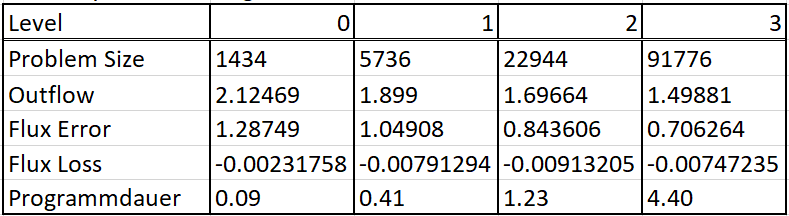
\includegraphics[width=0.99\textwidth]{../Aufgabe35/35_2_sym.png}}	 
\end{figure}


\begin{figure}[H]
	\centering
	\captionabove{non-symmetric}
	\subfigure{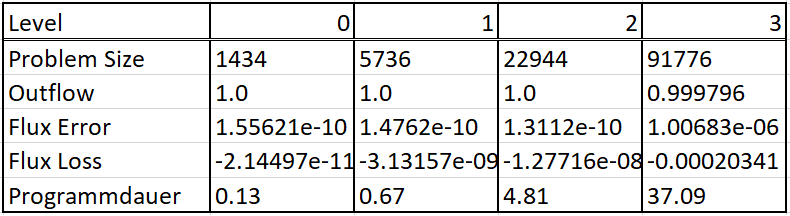
\includegraphics[width=0.99\textwidth]{../Aufgabe35/35_2_nonsym.png}}	 
\end{figure}

Wir wollen nun auf die Vor- und Nachteile bei symmetrischer und nicht-symmetrischer Konfiguration eingehen.
Schnell fällt ins Auge, dass die Ergebnisse des nicht-symmetrischen Verfahrens deutlich besser sind als mit symmetrischer Konfiguration. Während nämlich der Flux Error auf allen Leveln bei der symmetrischen Konfiguration nahe 1 ist, bewegen wir uns bei nicht-symmetrischer Konfiguration im Bereich von (sogar meist besser als) $10^{-6}$. Allerdings sieht man auch sehr schnell ein, dass dies nur auf Kosten der Programmdauer möglich ist. Während auf Level 3 der symmetrische Fall nur 4,4 Sekunden dauert, benötigt das nicht-symmetrische Verfahren sogar fast das 10-fache (ca. 40 Sekunden). 

\subsubsection{Aufgabe 35.3}
\begin{figure}[H]
	\centering
	\captionabove{deg = 2}
	\subfigure{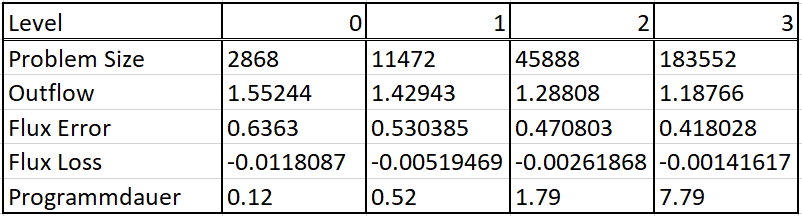
\includegraphics[width=0.99\textwidth]{../Aufgabe35/35_3_level.png}}	 
\end{figure}

Wie bei vorherigen Berichten berechnen wir auch hierzu mithilfe des Flux Errors eine Annäherung an die Konvergenzrate $p$ für den DG Ansatz mit quadratischen Ansatzelementen und symmetrischer Konfiguration.
Wir erhalten 
\begin{align*}
 \frac{e_l^{flux}}{e_{l+1}^{flux}} \approx 1.1508.
\end{align*}
Daraus erhalten wir die Konvergenzrate
\begin{align*}
  p \approx 0.2027.
\end{align*}

\subsubsection*{Penalty}
Wir betrachten nun den Einfluss des Parameters penalty auf das symmetrische DGV mit quadratischen Ansatzelementen.

\begin{figure}[H]
	\centering
	\captionabove{deg = 2, symmetrisch, level = 3}
	\subfigure{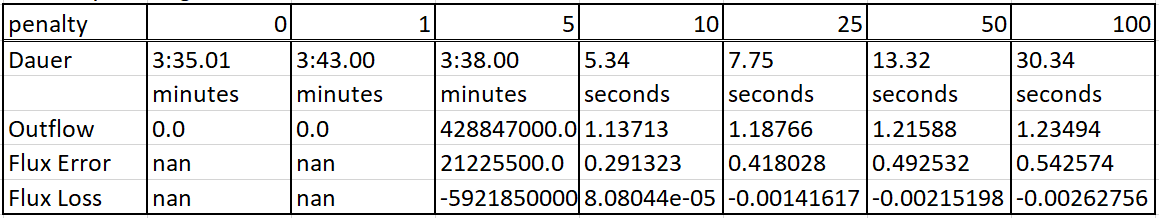
\includegraphics[width=0.99\textwidth]{../Aufgabe35/35_3_dauer.png}}	 
\end{figure}

Wie wir anhand der Tabelle sehen, ist das Verfahren für zu kleinen penalty instabil. Für penalty = 0,1,5 liefert das Verfahren keine brauchbaren Ergebnisse und benötigt eine lange Programmlaufzeit.
Für penalty = 10 erhalten wir eine gute Lösung bei relativ geringer Programmlaufzeit. Erhöhen wir nun den penalty noch weiter, so wird die Programmlaufzeit größer und zugleich die Lösung sogar schlechter. Es gilt also den penalty optimal in der Hinsicht zu wählen, dass das Verfahren stabil ist und der penalty trotzdem möglichst gering.



\subsubsection*{Problemgröße}
Wir wollen uns im Folgenden überlegen, wie die Anzahl der Unbekannten bei den unterschiedlichen Konfigurationen zustande kommen. 
Betrachten wir hierbei zunächst die FEM mit linearen Ansatzelementen stellen wir fest, dass sich die Problemgröße ungefähr in der Größenordnung der Anzahl der Knoten bewegt.
Wir können dies dadurch erklären, dass wir in unserem Ansatzraum für jeden Einzelknoten eine 'Hütchenfunktion' wählen können, welche einen Freiheitsgrad in der Gesamtapproximation ergibt.
Was wir allerdings noch beachten müssen, ist, dass die Dirichletränder bereits fest in unserem Ansatzraum $V_h(0)$ eingebaut sind, weswegen wir Knoten an Dirichleträndern nicht betrachten dürfen.
Es war uns leider nicht möglich die genaue Zusammensetzung der Problemgröße nachzuvollziehen. Was uns verwundert, ist, dass selbst auf verschiedenen Meshes mit gleich vielen Knoten bei gleichem Problem unterschiedliche Problemgrößen zustandekommen:
\begin{itemize}
  \item UnitSquare Lv4 = 289 (=Anzahl der Knoten)
  \item 2Triangles Lv4 = 321
  \item 8Triangles Lv3 = 353
  \item Square500  Lv0 = 342
\end{itemize} 
Sehr schön sieht man allerdings, dass wir pro Level ungefähr eine Vervierfachung der Problemgröße erhalten. Dies ist der Tatsache geschuldet, dass wir durch die Halbierung der Gitterweite viermal so viele Knoten erhalten.

Betrachten wir nun quadratische Ansatzelemente, erhalten wir auf Level 0 im Vergleich zu lineare Ansatzelementen ebenfalls etwa das Vierfache. Auch dies versuchen wir wieder anschaulich zu erklären: 
Wir können uns bei der Überlegung, wieviele Freiheitsgrade hinzukommen, einer einfachen Analogie bedienen: 
Durch die Wahl von quadratischen Ansatzelementen erhalten wir auf jeder Kante, also zwischen zwei Knoten, einen zusätzlichen Freiheitsgrad. Man kann also einsehen \textcolor{green}{??? BILD}, dass wir insgesamt in etwa so viele Freiheitsgrade erhalten, wie bei einem Gitter halber Gitterweite vorliegen. Das heißt wir erhalten beim Schritt von linearen zu quadratischen Ansatzelementen auch wieder ungefähr eine Vervierfachung des Ausgangswertes. Innerhalb der Diskretisierung mit quadratischen Ansatzelementen sehen wir erneut das Verhalten wie zuvor bei den linearen Ansatzelementen, d.h. eine Erhöhung des Levels um 1 hat eine Vervierfachung der Problemgröße zu folge.

\begin{figure}[H]
	\centering
	\captionabove{Problemgröße}
	\subfigure{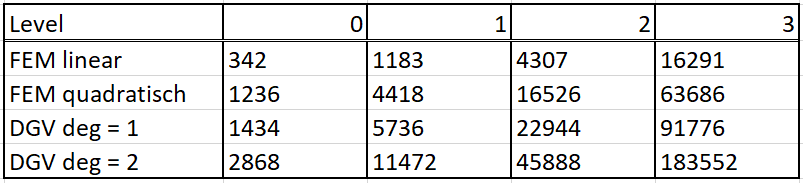
\includegraphics[width=0.99\textwidth]{../Aufgabe35/blub.png}}	 
\end{figure}

Betrachten wir nun das Discontinous Galerkin Verfahren. Wir müssen hierbei beachten, dass wir nun auch unstetige Ansätze erlauben. Es sind also auf den Knoten auch Sprungstellen erlaubt. Wir können uns auch hier einer einfachen Analogie bedienen und betrachten für jeden Knoten für jede anliegende Zelle einen eigenen Hilfsknoten. In unserem Fall erhalten wir bei linearen Ansatzelementen für jede Zelle gerade drei dieser Hilfsknoten (Square500 ist aus Dreiecken aufgebaut). Wir erhalten also für Level 0 (478 Zellen) gerade $3 \cdot 478 = 1434$ Freiheitsgrade. Mit steigendem Level erhalten dann exakt viermal so viele Freiheitsgrade, da bei Halbierung der Gitterweite sich die Zellenanzahl vervierfacht. 

Betrachten wir nun erneut den Schritt von deg = 1 auf deg = 2 können wir die gleiche Analogie wie bereits bei der FEM nutzen. Wir erhalten also bei den quadratischen Ansatzelementen jeweils auf den Kanten einen weiteren Freiheitsgrad. Nun ist aber auch dieser Parameter wieder unstetig wählbar. Mit dem gleichen Trick wie zuvor bei deg = 1 können wir uns also überlegen, dass wir nun auch für jede Kante für jede angrenzende Zelle einen Freiheitsgrad erhalten und so gerade auf das sechsfache der Zellenanzahl kommen (jede Zelle hat 3 Ecken und 3 Kanten).
Auch diese Werte lassen sich genau so in der Tabelle wiederfinden und wir können insgesamt die Verdopplung der Freiheitsgrade beim Schritt von deg = 1 auf deg = 2 feststellen.









\end{document}

